\documentclass[12pt,a4paper]{article}
\usepackage{amsmath,amscd,amsbsy,amssymb,latexsym,url,bm,amsthm}
\usepackage{epsfig,graphicx,subfigure}
\usepackage{enumitem,balance}
\usepackage{wrapfig}
\usepackage{mathrsfs,euscript}
\usepackage[usenames]{xcolor}
\usepackage{hyperref}
\usepackage{booktabs}
\usepackage{threeparttable}

\usepackage[vlined,ruled,linesnumbered]{algorithm2e}
\hypersetup{colorlinks=true,linkcolor=black}

\newtheorem{theorem}{Theorem}
\newtheorem{lemma}[theorem]{Lemma}
\newtheorem{proposition}[theorem]{Proposition}
\newtheorem{corollary}[theorem]{Corollary}
\newtheorem{exercise}{Exercise}
\newtheorem*{solution}{Solution}
\newtheorem{definition}{Definition}
\theoremstyle{definition}

\renewcommand{\thefootnote}{\fnsymbol{footnote}}

\newcommand{\postscript}[2]
 {\setlength{\epsfxsize}{#2\hsize}
  \centerline{\epsfbox{#1}}}

\renewcommand{\baselinestretch}{1.0}

\setlength{\oddsidemargin}{-0.365in}
\setlength{\evensidemargin}{-0.365in}
\setlength{\topmargin}{-0.3in}
\setlength{\headheight}{0in}
\setlength{\headsep}{0in}
\setlength{\textheight}{10.1in}
\setlength{\textwidth}{7in}
\makeatletter \renewenvironment{proof}[1][Proof] {\par\pushQED{\qed}\normalfont\topsep6\p@\@plus6\p@\relax\trivlist\item[\hskip\labelsep\bfseries#1\@addpunct{.}]\ignorespaces}{\popQED\endtrivlist\@endpefalse} \makeatother
\makeatletter
\renewenvironment{solution}[1][Solution] {\par\pushQED{\qed}\normalfont\topsep6\p@\@plus6\p@\relax\trivlist\item[\hskip\labelsep\bfseries#1\@addpunct{.}]\ignorespaces}{\popQED\endtrivlist\@endpefalse} \makeatother

\begin{document}
\noindent

%========================================================================
\noindent\framebox[\linewidth]{\shortstack[c]{
\Large{\textbf{Lab03-Greedy Strategy}}\vspace{1mm}\\
CS214-Algorithm and Complexity, Xiaofeng Gao, Spring 2021.}}


\begin{center}
\footnotesize{\color{red}$*$ If there is any problem, please contact TA Haolin Zhou.}\par
% Please write down your name, student id and email.
\footnotesize{\color{blue}$*$ Name:\_\_\_\_\_\_\_\_\_  \quad Student ID:\_\_\_\_\_\_\_\_\_ \quad Email: \_\_\_\_\_\_\_\_\_\_\_\_}
\end{center}

\begin{enumerate}
	\item \textit{Interval Scheduling.} Interval Scheduling is a classic problem solved by \textbf{greedy algorithm}: given $n$ jobs and the $j$-th job starts at $s_j$ and finishes at $f_j$. Two jobs are compatible if they do not overlap. The goal is to find maximum subset of mutually compatible jobs. Tim wants to solve it by sort the jobs in descending order of $s_j$. Is this attempt correct? Prove the correctness of such idea, or else provide a counter-example.

\begin{solution}

\textbf{The attempt is correct}.

Let $i_1,i_2, ...,i_k$ denote set of jobs selected by greedy, in an inverted order, which is to say $i_1$ is the last job and $i_k$ is the first job.

Similarly, let $j_1, j_2,...,j_m$ denote set of jobs in an optimal solution in an inverted order, with $i_1 = j_1, i_2=j_2,...,i_r=j_r$ for the largest possible value of $r$.

\textbf{Case 1:}

If $j_{r+1}$'s starting time is earlier than $i_{r+1}$,as showed in Fig.~\ref{case1}, then the optimal  choice should be the greedy one rather than this one, since the greedy choice will leave more time for the jobs before, which is more likely to have the most jobs. 

\begin{figure}[htbp]
    \centering
    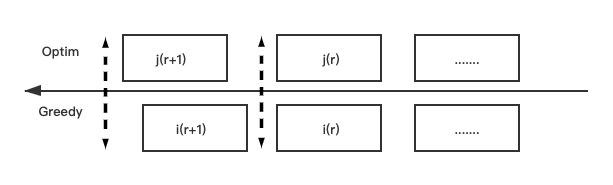
\includegraphics[width=0.6\textwidth]{case1.png}
    \caption{Case 1}\label{case1}
\end{figure}

\textbf{Case 2:}

If $j_{r+1}$'s starting time is later than $i_{r+1}$,as showed in Fig.~\ref{case2}, then the greedy choice should be the same as the optimal one rather than this one. It's because the algorithm selects the later starting time.

\begin{figure}[htbp]
    \centering
    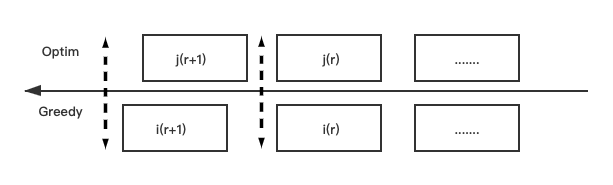
\includegraphics[width=0.6\textwidth]{case2.png}
    \caption{Case 2}\label{case2}
\end{figure}
\end{solution}

\textbf{In conclusion}, the optim is the same as the greedy. Therefore, the algorithm is optimal.	
	\item \textit{Done deal.} In a basketball league, teams need to complete player trades through matching contracts. Every player is offered a contract. For the sake of simplicity, we assume that the unit is $ M $, and the size of all contracts are integers. The process of contract matching refers to the equation: $ \sum_{i\in A} a_{i}=\sum_{j\in B} b_{j} $, where $ a_{i} $ refers to the contract value of player $ i $ in team $A$ involved in the trade and $ b_{j} $ refers to the value of player $ j $ in team $B$. 
	
	Assume that you are a manager of a basketball team and you want to get \textbf{one} star player from another team through trade. The contract of the star player is $ n (n\in \mathbb{N}^+) $. The goal is to complete the trade with as few players as possible. 
	
	\begin{enumerate}
		\item Describe a \textbf{greedy} algorithm to get the deal done with the least players in your team. Assume that there are only 4 types of contracts in your team: $25M$, $ 10M $, $ 5M $, $ 1M $, and there is no limit to the number of players. Prove that your algorithm yields an optimal solution.
		\item Suppose that the available contract sizes are powers of $c$,
		i.e., the values are $c^{0}, c^{1}, \ldots, c^{k}$ for some integers $c>1$ and $k \geq 1$. Show that the greedy algorithm always yields an optimal solution.
		\item Give a set of contract sizes for which the greedy algorithm does not yield an optimal solution. Your set should include a $ 1M $ so that there is a solution for every value of $ n $.
	\end{enumerate}
	
   \begin{solution}
   ~\\
   
   \begin{enumerate}
 
   \item
   The algorithm is showed in Alg.~\ref{alg greedy}. This is actually the same policy used in \textbf{Coin Changing} problem. In each turn we select the largest contract that is smaller than $n$ and finally we will get the deal.
   
   \begin{algorithm}[H]
   \caption{Greedy Algorithm}\label{alg greedy}
		Sort contracts denominations by value: $c_1=1, c_2=5, c_3=10, c_4=25$.\;
		$S\leftarrow \emptyset$\;
		$x\leftarrow n$\;
		\While{$x\neq0$}{
		let $k$ be largest integer such that $c_k < x$\;
		$x\leftarrow x-c_k$\;
		$S\leftarrow S\cup \{k\}$\;
		}
		\Return $S$\;
		
	\end{algorithm}
~\\	
\textbf{Theorem.}Greedy algorithm is optimal for Done Deal Problem.

\textbf{Proof.}

First we introduce several properties in this problem.
\begin{itemize}
\item \textbf{Property 1.} Number of $c_1\leq4$.

\textbf{Proof.} Replace 5 $c_1$ with 1 $c_2$.

\item \textbf{Property 2.} Number of $c_2\leq 1$.

\textbf{Proof.} Replace 2 $c_2$ with 1 $c_3$.

\item \textbf{Property 3.} Number of $c_3\leq2$.

\textbf{Proof.} Replace 3 $c_3$ with 1 $c_4$ and 1 $c_2$.

\item \textbf{Property 4.} Number of $c_2$ + Number of $c_3$ $\leq2$

\textbf{Proof.} From \textbf{Property 2 \& 3}, there is only one case not proved, which is Number of $c_2=1$ and Number of $c_3=2$.

Replace them with 1 $c_4$.

\end{itemize}

Second, we prove the algorithm is greedy.

(By induction on $n$)Consider an optimal way to deal with $c_k<n<c_{k+1}$ and the greedy sells the contract $c_k$. We claim that any optimal solution must also  sells the contract $c_k$.

If not, it needs enough contracts of type $c_1, ...,c_{k-1}$ to add up to $n$.

\begin{tabular}{|c|c|c|c|}
\hline
$k$ & $c_k$ & Restriction &Max value of contracts 1,2,..k-1 in any OPT\\
\hline
1 & 1 & Property 1 & -\\
\hline
2 & 5 &Property 1\& 2 &4\\
\hline
3 & 10 &Property 1\&2\&3\&4 & 4$\times$1+5= 9\\
\hline
4 & 25 &Property 1\&2\&3\&4 & 2$\times$10+4$\times$1=24\\
\hline
\end{tabular}

Then the problem reduces to deal with $n-c_k$, which, by induction, is optimally solved by greedy algorithm.

\item

\textbf{Proof:}


(By induction on $n$)Consider an optimal way to deal with $c^p<n<c^{p+1}, p=0,1,...k$ and the greedy sells the contract $c^p$. We claim that any optimal solution must also  sells the contract $c^p$.
~\\

\textbf{Property 1.} $ c^{p+1} \geq 2\times c^{p}$

\textbf{Proof.} Integer $c>1$ means $c\geq2$. So $c^{p+1}=c^p\times c\geq 2\times c^p$.
~\\

If the optimal solution doesn't select $c^p$, then it needs enough contracts to sum up to $n$. From \textbf{Property 1}, we know that it at least needs 2 contract $c^{p-1}$ to compensate for not selecting $c^p$. This is unvoidable because it can not use $c^{p+1}$. Therefore, the optimal solution must select $c^p$, which is greedy.

Then the problem reduces to deal with $n-c^p$, which, by induction, is optimally solved by greedy algorithm.

\item
The set can simply be: $\{1M, 6M, 10M, 25M\}$.

For example, if $n=12$:

By $Greedy\ Algorithm$, the contract set would be $\{10M, 1M, 1M\}$.

However, the optimal solution is $\{6M, 6M\}$.

\textbf{Explanation:}

By my observation, if the element of the contracts does not satisfy \textbf{Property 1} in the \textbf{problem b}(shown below), the greedy algorithm can not work. 

~\\
\textbf{Property 1.} $c_{k+1}\geq 2\times c_{k}$
~\\

The intuitive proof is shown in Fig.~\ref{explain}. If $c_k$ and $c_{k+1}$, two adjacent contracts, can not satisfy a relationship that is shown in \textbf{Property 1}, the greedy choice may fail to reduce the total number of contracts. In Fig.~\ref{explain}, the left is when the greedy algorithm works and the right is when it does not work. When $c_k$ and $c_{k+1}$ can not satisfy \textbf{Property 1}, the greedy algorithm needs at least one contract to replace two $c_k$, possibly two or more. \textbf{This is not optimal.}



\begin{figure}[htbp]
    \centering
    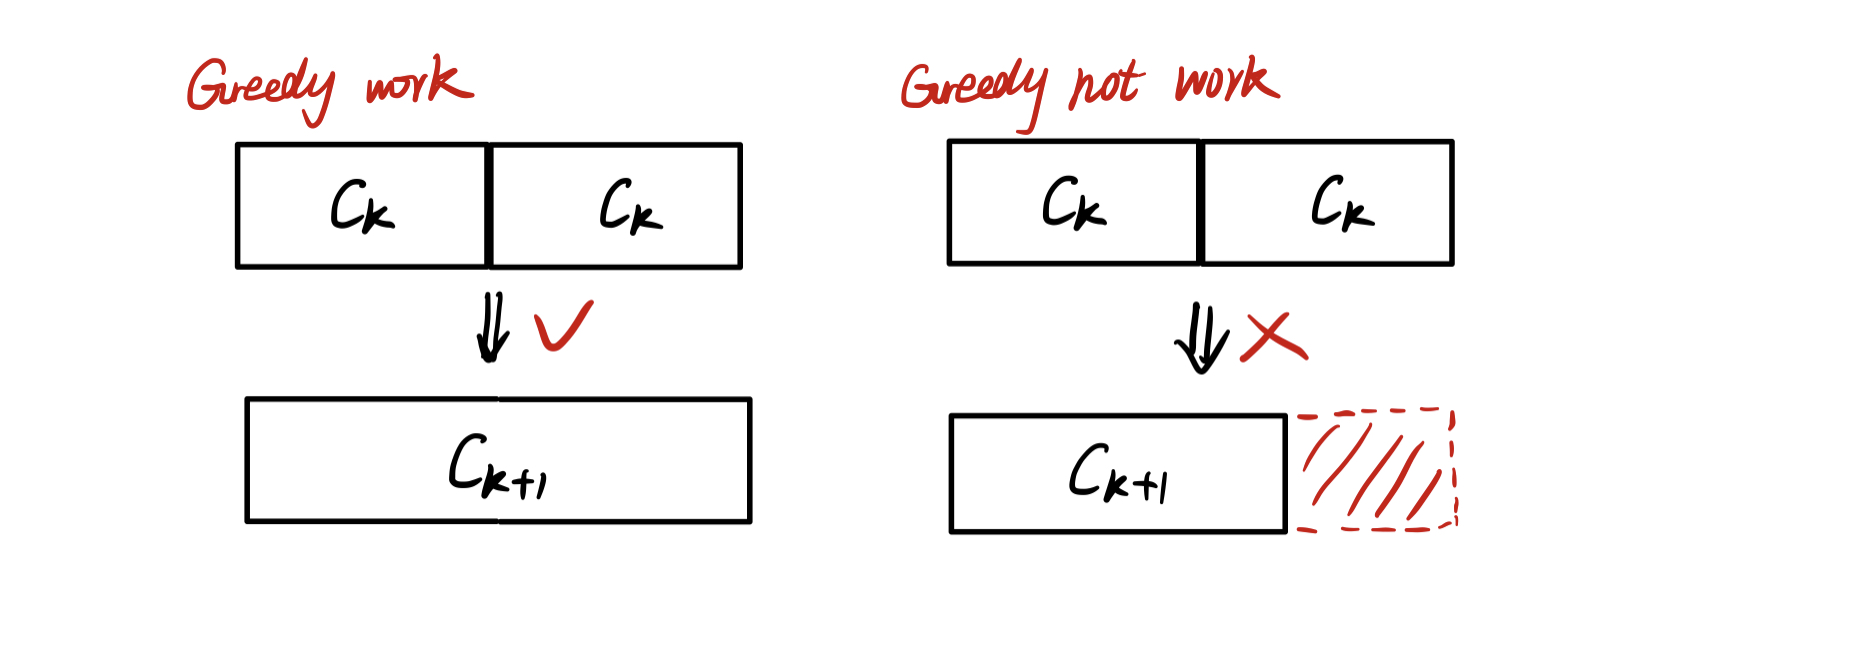
\includegraphics[width=0.6\textwidth]{explain.jpg}
    \caption{When Greedy Algorithm Works?}\label{explain}
\end{figure}

\end{enumerate}
    \end{solution}
	
    \item \textit{Set Cover.} \textbf{Set Cover} is a typical kind of problems that can be solved by greedy strategy. One version is that: Given $n$ points on a straight line, denoted as $\{x_i\}_{i=1}^n$, and we intend to use minimum number of closed intervals with fixed length $k$ to cover these $n$ points.
    \begin{enumerate}
    	\item Please design an algorithm based on \textbf{greedy} strategy to solve the above problem, in the form of \emph{pseudo code}. Then please analyze its \emph{worst-case} complexity.
    	\item Please prove the correctness of your algorithm.
    	\item Please complete the provided source code by C/C++ {\color{blue}(The source code \emph{Code-SetCover.cpp} is attached on the course webpage)}, and please write down the output result by testing the following inputs: 
    	\begin{enumerate}
    		\item the number of points $n=7$;
    		\item the coordinates of points
    		$x=\{1,2,3,4,5,6,-2\}$;
    		\item the length of intervals
    		$k=3$.
    	\end{enumerate}
        \textbf{Remark}: Screenshots of running results are also acceptable 
    \end{enumerate}
    
   \begin{solution}
   
\begin{enumerate}
\item
~\\
The algorithm.~\ref{alg cover} \textbf{Greedy Cover Set} takes greedy strategy. To make the number of intervals small as far as possible, each interval begins at a point. This algorithm is intuitively like \textbf{Sliding Window}.

\begin{algorithm}[H]
   \caption{Greedy Cover Set}\label{alg cover}
		Sort Input points' coordinates by increasing order:$\{a_1, a_2,...,a_n\}$\;
		$i:=1, num:=0$\;
		\While{$i<n$}{
		$\{a_i, a_{i+1},...,a_{i+m}\} = interval[a_i, a_i+k]\ cover$\;
		$num++ $\;
		$i:=i+m$\;
		\If{$i==n$}{
		\Return num\;
		}
		$i++$\;
		\If{$i==n$}{
		\Return num+1\;
		}
		}
	\end{algorithm}
\end{enumerate}
 \end{solution}

\item

\item


\end{enumerate}



\vspace{20pt}

\textbf{Remark:} You need to include your .pdf and .tex files in your uploaded .rar or .zip file.

%========================================================================
\end{document}
